% !TeX engine = xelatex
% !TeX spellcheck = en-US
% adjust to 16:9 for displays. you can just use \documentclass[handout]{ctexbeamer} for notes

\documentclass[aspectratio=169]{beamer}
\usepackage{booktabs}
\usepackage{svg}
\usepackage{fontawesome}
\usepackage[style=authortitle-comp,backend=bibtex]{biblatex}
\usecolortheme{seagull}
\setbeamertemplate{sidebar right}{}
\setbeamertemplate{footline}{%
	\hfill\usebeamertemplate***{navigation symbols}
    \hspace{1cm}\insertframenumber{}/\inserttotalframenumber}

    \newcommand{\red}[1]{{\color{red}{#1}}}
    \newcommand{\blue}[1]{{\color{blue}{#1}}}

\title{Understanding, Detecting and Localizing Partial Failures in Large System Software\footfullcite{lou2020understanding}}
\date{\today}

\addbibresource{ref.bib}

\begin{document}

\begin{frame}
    \titlepage
\end{frame}

\begin{frame}{Overview}
    \tableofcontents
\end{frame}

\section{Problem definition}

\begin{frame}
    \frametitle{What is a Partial Failure?}
    \framesubtitle{An Example}
    \begin{center}
        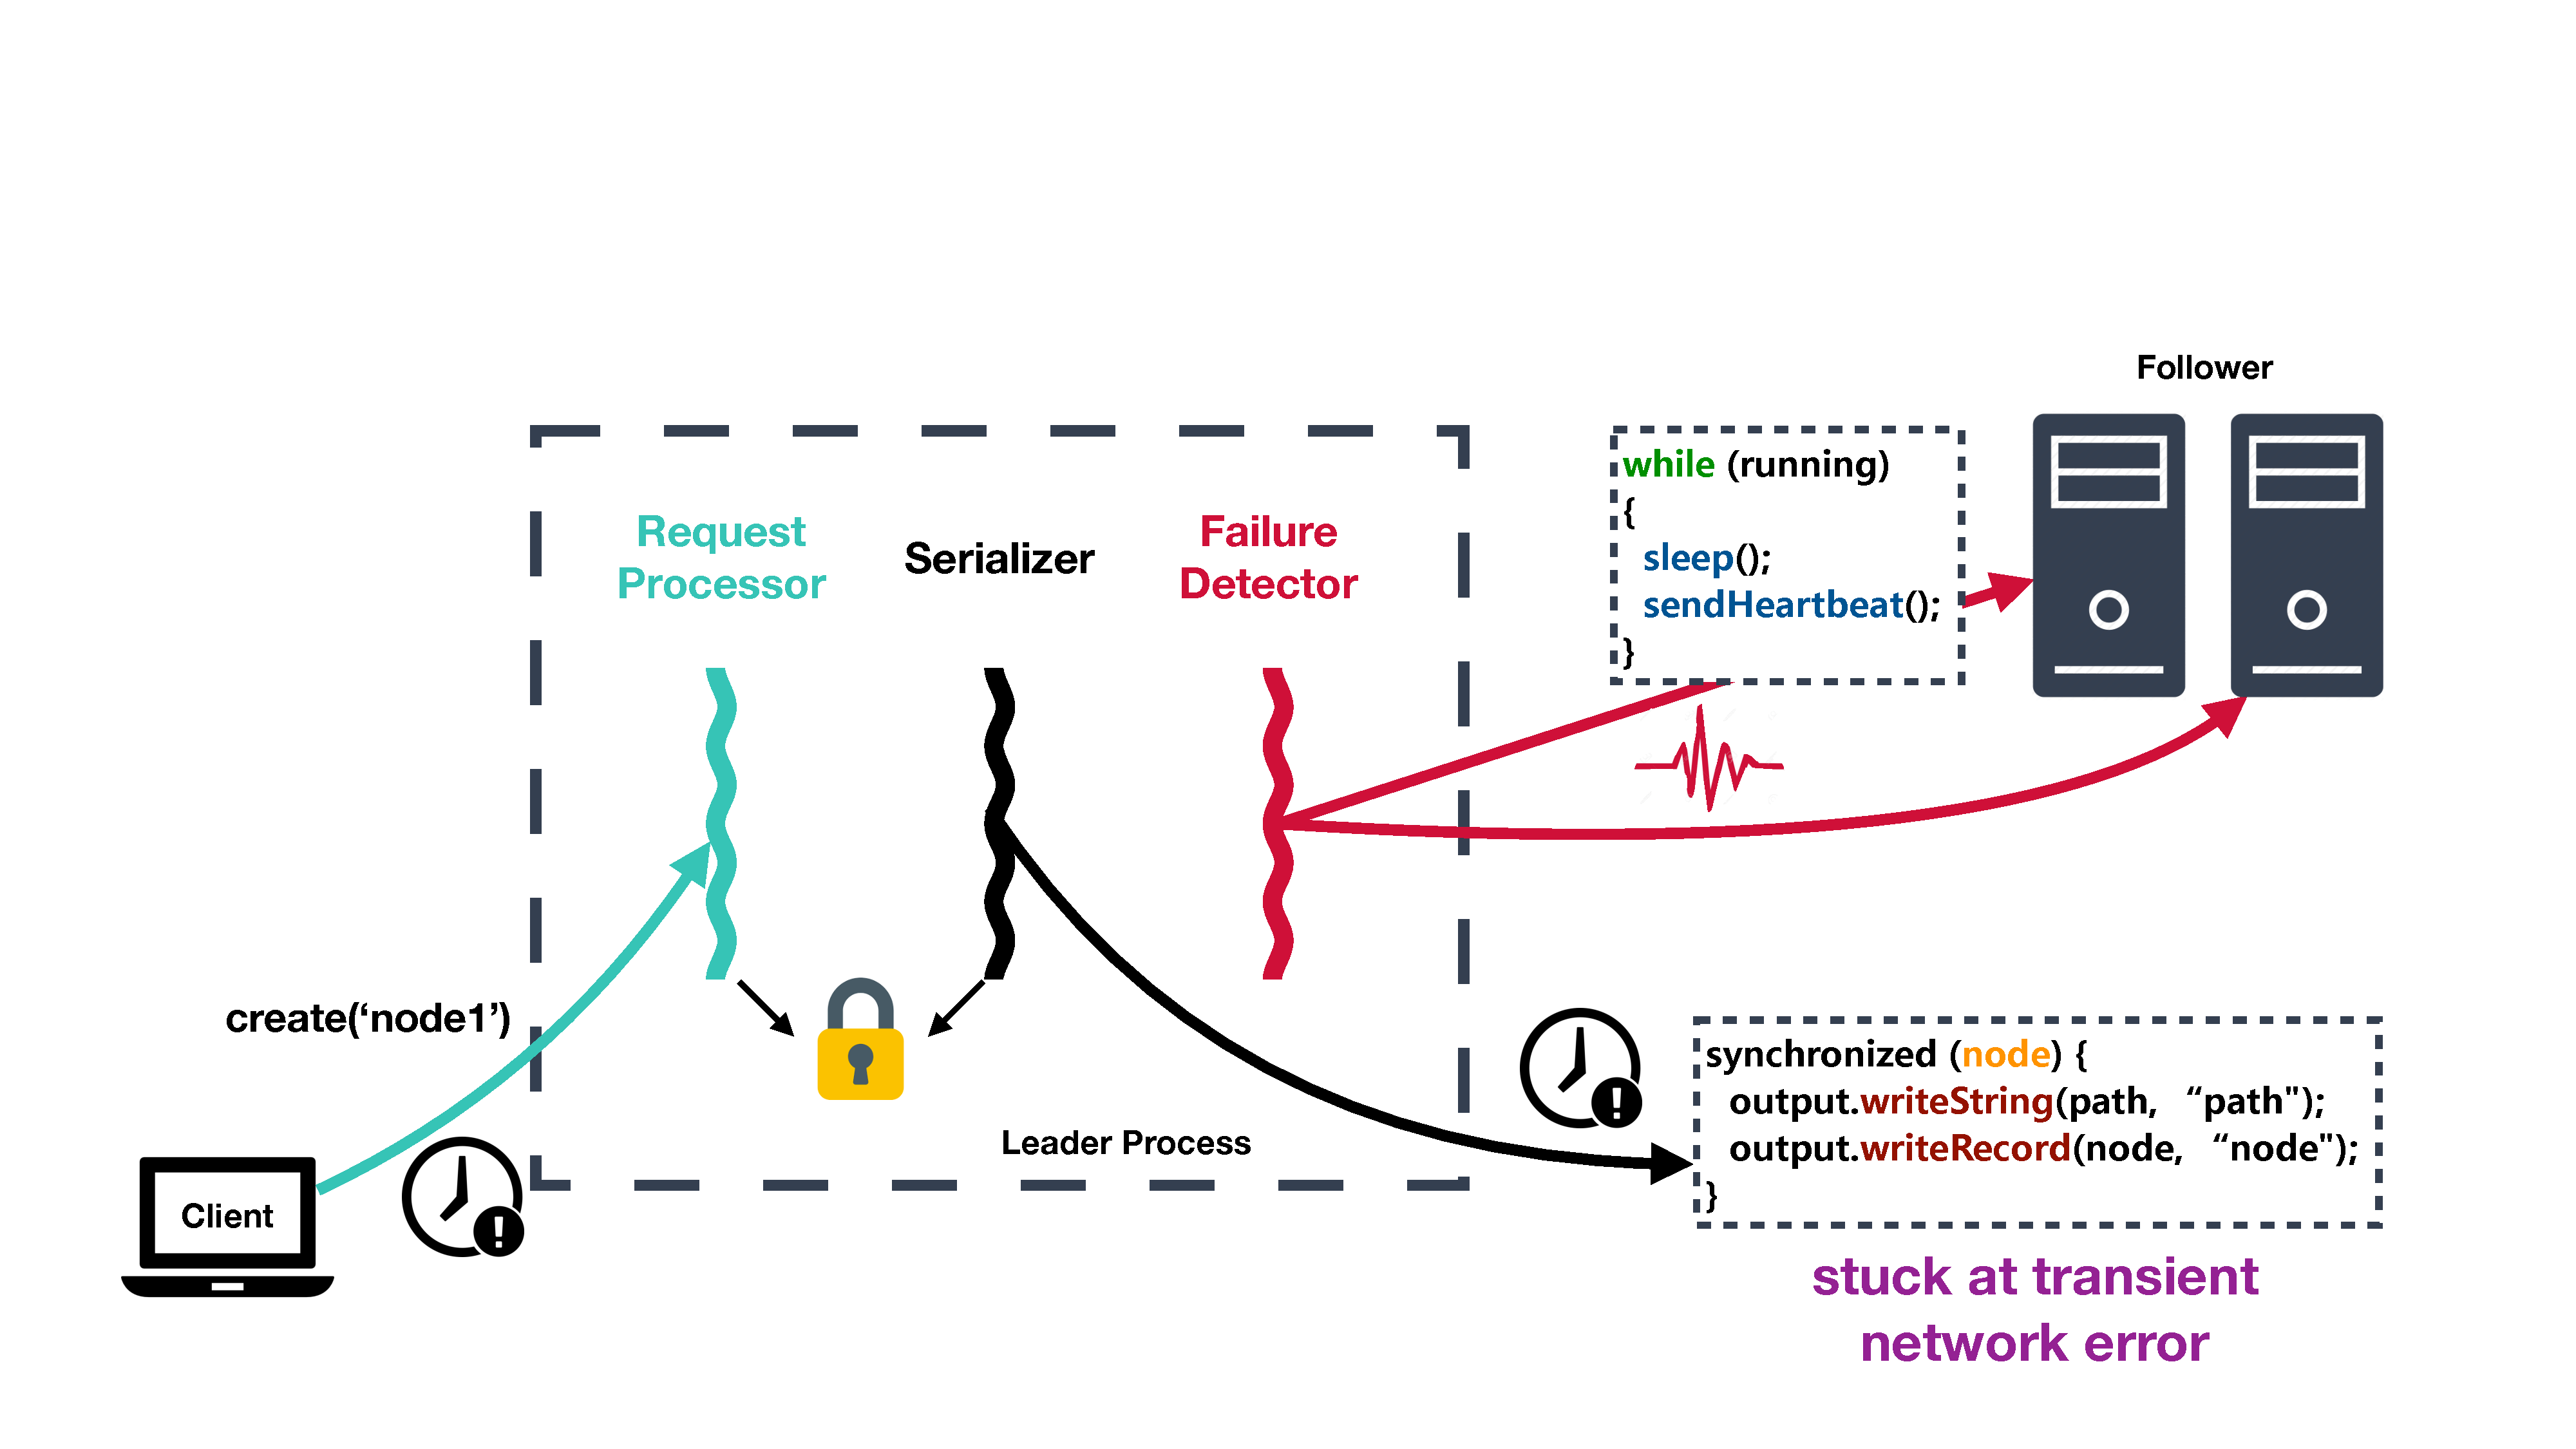
\includegraphics[width=\textwidth]{fig/example1}
    \end{center}
\end{frame}

\begin{frame}
    \frametitle{What is a Partial Failure?}
    \begin{definition}
        A partial failure is, in a process $\pi$ to be when a fault \textbf{does not} crash $\pi$ but causes safety or liveness violation or severe slowness for some functionality $R_f \subsetneq  R$

    \end{definition}
    \textbf{Scope:} In this paper, we will specify the partial failure at the \red{process} granularity instead of \blue{service}.
    \begin{center}
        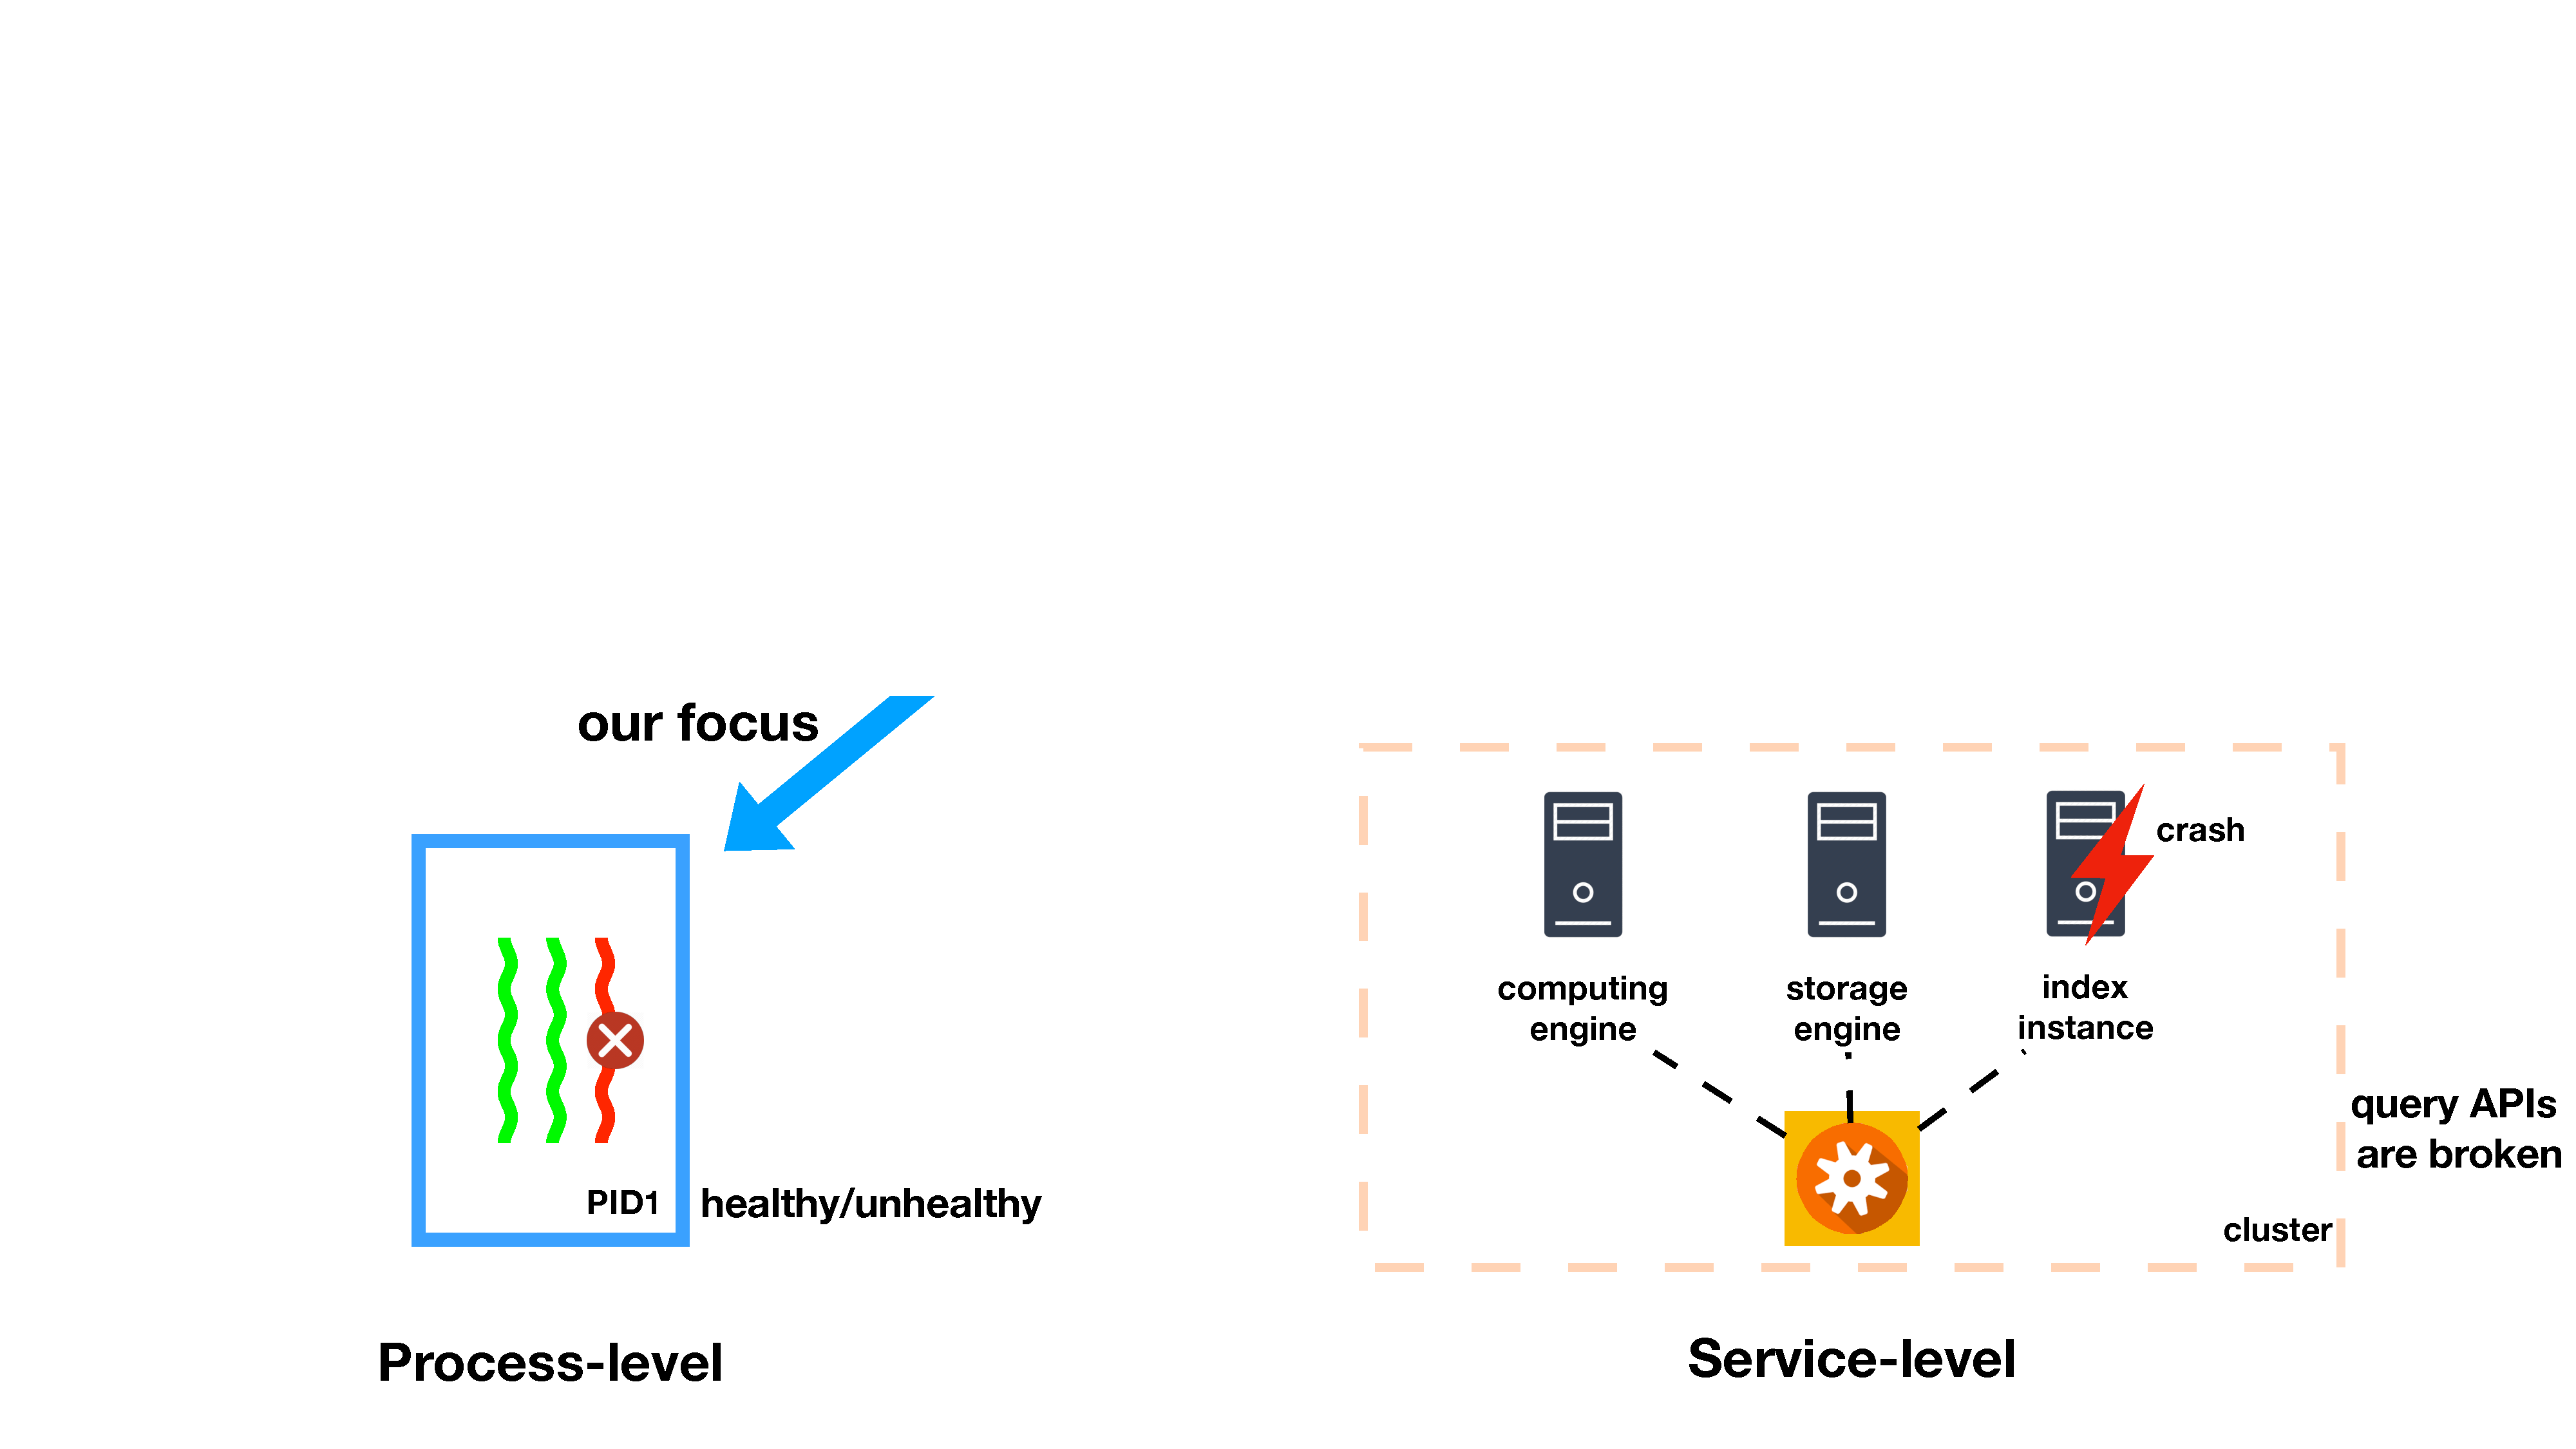
\includegraphics[width=.9\textwidth]{fig/level}
    \end{center}
\end{frame}

\section{Case Study}
\begin{frame}
    \frametitle{Study methodology}
    \begin{block}{\textbf{100 partial failure cases from five large, widely-used software systems}}
        \begin{itemize}
            \item Crawl all bug tickets tagged with critical priorities in the official
                  bug trackers
            \item Filter tickets from testing and randomly
                  sample the remaining failures tickets.
        \end{itemize}
    \end{block}

    Interestingly, \red{54\%} of them occur in the most recent \red{three} years’ software
    releases \textit{(average lifespan of all systems is \red{9} years)}
    \begin{center}
        \begin{tabular}{|c|c|c|c|c|}
            \toprule
            Software  & Language & Cases & Versions           & Date Range            \\
            \midrule
            ZooKeeper & Java     & 20    & 17 (3.2.1–3.5.3)   & 12/01/2009–08/28/2018 \\
            \hline
            Cassandra & Java     & 20    & 19 (0.7.4–3.0.13)  & 04/22/2011–08/31/2017 \\
            \hline
            HDFS      & Java     & 20    & 14 (0.20.1–3.1.0)  & 10/29/2009–08/06/2018 \\
            \hline
            Apache    & C        & 20    & 16 (2.0.40–2.4.29) & 08/02/2002–03/20/2018 \\
            \hline
            Mesos     & C++      & 20    & 11 (0.11.0–1.7.0)  & 04/08/2013–12/28/2018 \\
            \bottomrule
        \end{tabular}
    \end{center}
\end{frame}

\end{document}